% Set document type
\documentclass[conference]{IEEEtran}

% Packages
\usepackage{graphicx}
%\usepackage{flushend}
\usepackage{cite}
\usepackage{mathtools}
\usepackage{subfigure}
% For highlighting areas to revise, use color package
\usepackage{color}

% TODO command
\newcommand {\todo}[1] {\textcolor{red}{#1}}

% Fix hyphenation of words
\hyphenation{op-tical net-works semi-conduc-tor}

% Start document, set bibliography
\begin{document}
\bibliographystyle{plain}

% Create title and author block
\title{Stencil Code Optimization for GPUs Through Machine Learning}
\author{\IEEEauthorblockN{Adam Barker}
\IEEEauthorblockA{University of Colorado at Colorado Springs\\
abarker2@uccs.edu}}
\maketitle

% Abstract
\begin{abstract}
	\todo{Add a reference to the tuning framework in here.}
	The microprocessor field today has begun to reach its limits as power and thermal constraints have been met and no longer can much leverage of increasing the processor's clock speed be achieved. Thus, much of the scientific and engineering community has shifted to using many-core architectures, such as GPUs, in order to do parallel computations. This paper focuses on the use of genetic algorithms to guide the optimization of stencil codes on NVIDIA's Compute Unified Device Architecture (CUDA) based GPUs and GPGPUs. In particular, we have implemented two separate stencil kernels (Jacobi 7 point and 27 point) in CUDA with each implementation parameterized for several optimiation parameters (thread blocking and loop unrolling factors). We then used a genetic algorithm\cite{DEAP} to find optimal configurations for each kernel. Our results show that this approach is capable of generating near-optimal configurations in a much more timely fashion than exhaustive search.

\end{abstract}

a
\section{Introduction}
	As microprocessors reach the power wall, benefits of increasing the clock frequency are no longer achieveable as the cost to system stability and cooling is too much to warrant the increase in performance\cite{landscape}. This has shifted the focus of the parallel community to many-core architectures, such as those found in Graphical Processing Units (GPUs), as they are comprised of a few hundred or thousand simple cores that are capable of performing highly-parallel computations with much more throughput than a typical multi-core system. However, developing parallel algorithms for GPUs can be no simple task for developers as developers must have a firm understanding of the underlying architecture and hardware properties in order to correctly write programs that correctly take advantage of these properties. Thus, there is a desire to develop a method to automatically apply optimizations to GPU programs in order to avoid the necessity of understanding the complexities of the hardware and architecture of the system.

	Recently, in order to meet this desire, researchers have devloped several methods in order to automatically tune or automatically generate optimized codes for both GPUs and multi-core systems. However, as more optimizations are discovered, the search space the auto-tuner must search through grows to an amount where auto-tuning is no longer viable as the number of possible combinations of parameters becomes too large to effectively search through. This then sets the perfect stage for a machine learning application to predict the optimal code instead as it does not have to go through the entire search space, but rather make predictions based on previous results.
	b

%\todo{Reference GPUs in this paragraph, go into more detail.}
	This work presents a method to use genetic algorithms in order to discover optimized configurations of parameterized CUDA stencil (nearest-neighbor) codes -- a class of algorithms that typically work in structured grids to perform computations, such as finite-difference methods for solving parital differential equations, on a node within the grid by doing computations on the neighbors around the given node. Our work focuses on a simple 3D heat equation using two different stencil codes as the training set for a genetic algorithm to search through a search space of several thousand combinations of possible optimization parameters. Although stencil codes are important as scientific computations, they also provide a unique opportunity for hardware benchmarking as they are computationally simple and require a large use of memory, allowing for benchmarking of instruction-level and data-level parallelism\cite{Datta}. These codes greatly benefit being run on GPUs as the parallel forms of these codes contain a great deal of instruction level parallelism which translates well to SIMD architectures, which are present on GPUs.

\begin{figure*}[ht]
	\centering
	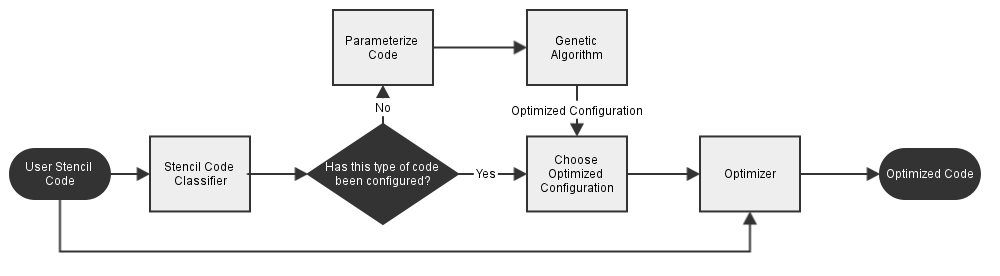
\includegraphics[width=\linewidth]{auto-tuning_framework.png}
	\caption{Overview of auto-tuning framework}
\end{figure*}

	\todo{Talk about the tuning framework as a whole and that your research is a validation tool of the framework (feasability study) so that your research appears more complete.}
	This research is the development of the optimal configuration generator portion of the framework detailed in Figure 1. The auto-tuning framework will be used to optimize existing stencil codes using machine learning in order to predict optimal tuning parameters that will be given to the optimizer which will apply these optimizations to the given stencil code and then output the optimized version of the given code. This is done so that developers can easily write unoptimized code for use in their programs and then run this auto-tuning framework on their code in order to use optimized code that correctly fits within their existing program.

	%\todo{Expand this sentence: In particular, we have implemented three separate stencil kernels (Jacobi 7 point, 25 point, and 27 point) in CUDA with each implementation parameterized for several optimiation parameters (thread blocking and loop unrolling factors). into a paragraph, along with description of genetic algorithms.}
	In order to train the machine learning portion of the configuration generator, we implemented two stencil kernels to be used across three separate GPUs. The stencil codes we implemented were a 7 point and 27 point Jacobi iterative stencil codes and then parameterized the relevant optimizations that the genetic algorithms would find configurations for so that the fitness test for the genetic algorithm could change these parameters easily before compiling and running.

	%\todo{REVISE: make sure this paragraph is consistent with last sentence of the abstract.}
	The optimization parameters considered for the generation of the search space that we used were the number of threads to use in the computation, and the distance to unroll the inner loop in our code. This inner-loop arises from our use of 2.5D blocking, a thread blocking optimization that allows for threads to only be launched in a single plane of the 3D data, and then stream through the remaining axis as the computation goes on. This search space consists of 60 different thread configurations and 192 different loop unrolling configurations, giving us a search space of 11,520 possible combinations. Although the size of this search space is relatively small for most machine learning applications, one must consider the time it takes to compile the code as on our system, typical complilation time is 3 seconds, meaning that an exhaustive search through the search space would take more than 9 hours, whereas our use of a genetic algorithm took on average 8 minutes to find an optimized configuration.

%	\todo{List the structure of the rest of the paper. (The rest of the paper is organized as follows:...}
	The rest of the paper is organized into four sections: related work, tuning framework, experimental results, and conclusions and future work. In related work, other research that has been done in the field is presented and summarized along with how it is utilized in this research. The tuning framework section goes into more detail of stencil codes, optimizations, and the genetic algorithm that we used. Experimental results includes the experimental setup and the results we obtained from running our implementation on three different systems as well as a discussion of these results. Conclusions and future work summarizes this research and presents the outlook of incorporating it into future work.

\section{related work}
	\todo{Revise this section so that it contains NO future tense as well as includes more details on all of the works that are used in this research.}
	The current state of stencil code research is most researchers are focused primarily on either manual optimization of the codes or creating auto-tuning tools to automatically input correctly optimized configurations for stencils. Datta et all have demonstrated the usefulness of both manual optimizations and auto-tuning techniques as a means to effectively optimize stencil codes on both cpus and gpus\cite{Datta}. This paper provides an effective base for retrieving optimizations as gana et all cite this work as their basis for using machine learning to optimize cpu stencil codes. They used genetic algorithms in combination with the kcca algorithm to perform quick searches through the parameter space\cite{gana}. Zhang et all also researched auto-tuning and auto-generation of optimized stencil codes specifically for gpus and gpu clusters which provides a more specific list of optimizations that are specifically used for gpu stencil code optimizations that we can use in this research\cite{zhang}. In terms of advanced manual optimizations for gpu stencil codes, nguyen et all provided a state-of-the art stencil code optimization that uses a combination of 2.5d thread blocking combined with 1d temporal blocking to create what they have called "3.5d" blocking which provides throughput increases on gpus of about two times what prior research had claimed\cite{nguy}. This research can be parameterized by changing the amount of temporal blocking to perform, thus allowing a search space to be created for this optimization to incorporate into this research.
	
\section{Tuning Framework}
	\subsection{Stencil Codes}
	Stencil codes are primarily used to solve paritial differential equations in order to perform simulations such as heat flow or electromagnetic field propogation\cite{Datta}. Most methods for solving these partial differential equations use iterative sweeps through spatial data, performing nearest-neighbor computations which are called stencils. Each node in the computation is weighted based on distance from the central node, which allows for the solving partial differential equations by switching these weights for the coefficients used in the solver. Using this structure, methods are created for different types of partial differential equation solvers such as Jacobi iterative methods, which are the stencil codes we used in this research.

\begin{figure}[h]
	\centering
	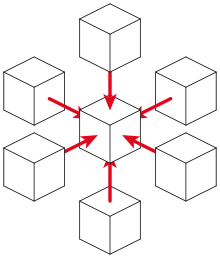
\includegraphics[width=5cm]{stencil-7.png}
	\caption{A 6-point Von-Neuman stencil (credit: wikipedia.org)}
\end{figure}
	As the data sizes used for stencil computations typically range outside the size of available cache memory, there is a large emphasis on data reuse and data-level parallelism in order to fully optimize stencil codes.

	Auto-tuning of stencil kernels has become a fairly large area of study in order to work around the necessity of knowledge of the low-level specifications of the architecture in order to optimize the kernel. However, these auto-tuners may have to look in a parameter space that is upwards of 40 million	combinations that may take months to fully check every single one for optimal performance\cite{Datta}. This then creates a demand for a faster optimization process that is still automated in order to create a process that is viable for industry use. Thus, machine learning may be a good option for automatic optimization as it can use reinforcement learning paired with statistical machine learning and genetic algorithms in order to explore the parameter space much faster. Using machine learning may also overcome another downfall of auto-tuning in that each auto-tuner is generally programmed for one architecture, whereas a learner can learn architectures as well and correctly optimize for them.	

%\section{Motivation}
%\todo{Move this section to second paragraph of the introduction.}
%	Due to the large number of optimizations to be considered, difficult architecture layouts to master, and constantly changing hardware, machine learning is a desirable approach to automatically optimizing stencil kernels quickly on any architecture. This would then allow for more advanced simulations to be done as they are no longer constrained by the difficulty to optimize stencil codes and programmers will no longer need to have a deep understanding of the underlying architecture in order to optimize stencil codes quickly and efficiently. This research will hopefully provide a framework to create a machine learning technique to optimize stencil kernels on advanced GPU and GPGPU architectures.

\subsection{Optimizations}

\subsection{Genetic Algorithms}

\section{Experimental Results}
\todo{Start with goal, then setup, then results}
The setup we used to perform the experiments on consisted of three GPUs: one GPGPU (Tesla C2050) and two standard GPUs (GTX 480, 680). Figure 3 details the theoretical peak FLoating-point OPeration rate (FLOP) determined by the number of cores ($\alpha$) multiplied by the clock rate of each code ($\delta$) multiplied by the number of FLOPs that can be performed each clock cycle ($\gamma$).
\begin{figure}[h]
	\centering
	$\alpha\times\delta\times\gamma$
	\caption{Theoretical peak FLOP rate equation.}
\end{figure}

\begin{figure}[h]
	\begin{center}
		\begin{tabular}
		{|c|c|c|}
			\hline
			GPU & Architecture & Peak FLOP rate\\
			\hline
			GTX 480 & Fermi & 1344 GFLOP/s\\
			Tesla C2050 & Fermi & 1030 GFLOP/s\\
			GTX 680 & Kepler & 3250 GFLOP/s\\
			\hline
		\end{tabular}
	\end{center}
	\caption{Peak GFLOP rate of GPUs (single precision)}
\end{figure}

	Four experimental data sets will be generated for the machine learning algorithm to use. These data sets will consist of a few thousand randomly-configured stencil codes which can be used by the machine learner in order for it to be able to select a set of optimizations to perform on the given kernel so that the kernel can be as optimized or nearly as optimized as a hand-optimized kernel. The four data sets will be created from two different stencil kernels which are:
	
\begin{itemize}
	\item A 7-point 3D Jacobi stencil. (8 FLOPs/node)
	\item A 27-point 3D Jacobi stencil. (31 FLOPs/node)
\end{itemize}

	Due to the wide variety of FLOPs/node of each stencil, this should allow us to verify the accuracy and usefulness of the machine learning algorithm in this research.

	These stencil kernels will be ran through a script to go through some combinations within the search space in order to form the initial population for the training set for the machine learner to traverse through. This process will take a long time as each combination requires a re-compile of the code and a run in order to gather the data from the NVIDIA CUDA profiling utility. While the data is being collected, other optimizations can be explored and the machine learner may be able to look at preliminary data as it is collected to perform some pre-tuning before it is given the entire training set.

\begin{figure}[h!]
	\centering
$a_{i,j,k}^{n+1} = \beta(a_{i,j,k}^n + a_{i\pm1,j,k}^n + a{i,j\pm1,k}^n + a_{i,j,k\pm1}^n)$
	\caption{7-point Jacobi stencil equation.}
\end{figure}

	The equation in figure 2 details a typical 7-point Jacobi stencil where a is the input grid, n is the iteration, and $\beta$ is the modifier to be applied to the neighborhood sum.
	
	\begin{figure*}[t]
\centering
	\subfigure[Tesla C2050 7 point]{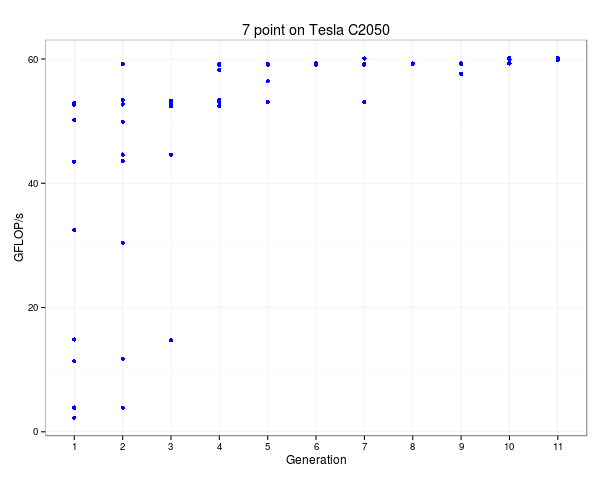
\includegraphics[width=0.4\linewidth]{gen7_C2050.png}}
	\label{fig:sub1}
	\hfill
	\subfigure[Tesla C2050 27 point]{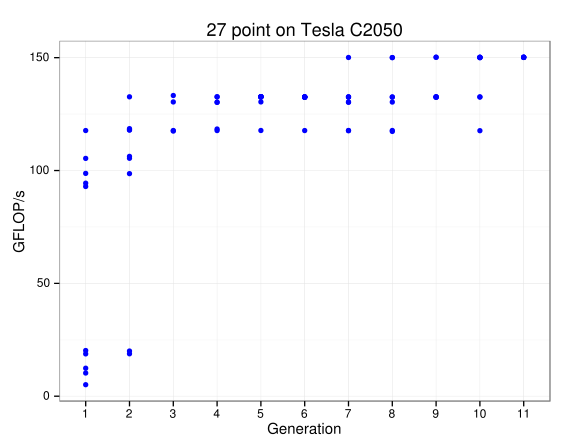
\includegraphics[width=0.4\linewidth]{gen27_C2050.png}}
	\label{fig:sub2}
	\hfill
	\subfigure[GTX 480 7 point]{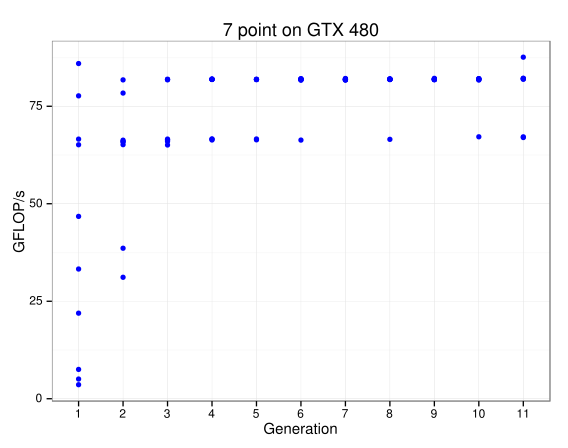
\includegraphics[width=0.4\linewidth]{gen7_480.png}}
	\label{fig:sub3}
	\hfill
	\subfigure[GTX 480 27 point]{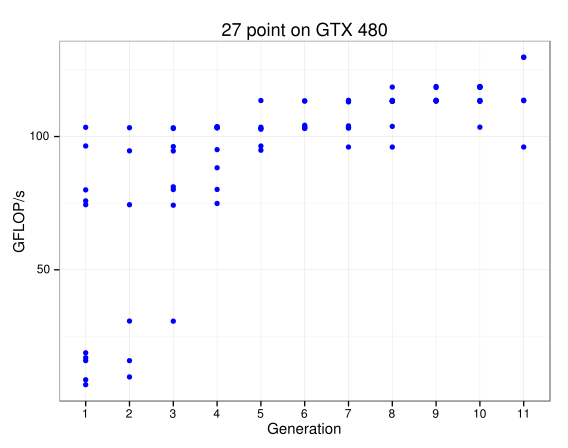
\includegraphics[width=0.4\linewidth]{gen27_480.png}}
	\label{fig:sub4}
	\caption{Results of genetic algorithm exploring configuration search space for different stencil kernels on different GPUs.}
\end{figure*}

\section{Conclusions and Future Work}

\section*{Acknowledgements}
\begin{center}
	This research is supported by NSF grant 1359275.
\end{center}

% Create References section
\bibliography{myBib}

% That's all folks
\end{document}
